\documentclass[twoside]{book}

% Packages required by doxygen
\usepackage{fixltx2e}
\usepackage{calc}
\usepackage{doxygen}
\usepackage[export]{adjustbox} % also loads graphicx
\usepackage{graphicx}
\usepackage[utf8]{inputenc}
\usepackage{makeidx}
\usepackage{multicol}
\usepackage{multirow}
\PassOptionsToPackage{warn}{textcomp}
\usepackage{textcomp}
\usepackage[nointegrals]{wasysym}
\usepackage[table]{xcolor}

% Font selection
\usepackage[T1]{fontenc}
\usepackage[scaled=.90]{helvet}
\usepackage{courier}
\usepackage{amssymb}
\usepackage{sectsty}
\renewcommand{\familydefault}{\sfdefault}
\allsectionsfont{%
  \fontseries{bc}\selectfont%
  \color{darkgray}%
}
\renewcommand{\DoxyLabelFont}{%
  \fontseries{bc}\selectfont%
  \color{darkgray}%
}
\newcommand{\+}{\discretionary{\mbox{\scriptsize$\hookleftarrow$}}{}{}}

% Page & text layout
\usepackage{geometry}
\geometry{%
  a4paper,%
  top=2.5cm,%
  bottom=2.5cm,%
  left=2.5cm,%
  right=2.5cm%
}
\tolerance=750
\hfuzz=15pt
\hbadness=750
\setlength{\emergencystretch}{15pt}
\setlength{\parindent}{0cm}
\setlength{\parskip}{3ex plus 2ex minus 2ex}
\makeatletter
\renewcommand{\paragraph}{%
  \@startsection{paragraph}{4}{0ex}{-1.0ex}{1.0ex}{%
    \normalfont\normalsize\bfseries\SS@parafont%
  }%
}
\renewcommand{\subparagraph}{%
  \@startsection{subparagraph}{5}{0ex}{-1.0ex}{1.0ex}{%
    \normalfont\normalsize\bfseries\SS@subparafont%
  }%
}
\makeatother

% Headers & footers
\usepackage{fancyhdr}
\pagestyle{fancyplain}
\fancyhead[LE]{\fancyplain{}{\bfseries\thepage}}
\fancyhead[CE]{\fancyplain{}{}}
\fancyhead[RE]{\fancyplain{}{\bfseries\leftmark}}
\fancyhead[LO]{\fancyplain{}{\bfseries\rightmark}}
\fancyhead[CO]{\fancyplain{}{}}
\fancyhead[RO]{\fancyplain{}{\bfseries\thepage}}
\fancyfoot[LE]{\fancyplain{}{}}
\fancyfoot[CE]{\fancyplain{}{}}
\fancyfoot[RE]{\fancyplain{}{\bfseries\scriptsize Generated by Doxygen }}
\fancyfoot[LO]{\fancyplain{}{\bfseries\scriptsize Generated by Doxygen }}
\fancyfoot[CO]{\fancyplain{}{}}
\fancyfoot[RO]{\fancyplain{}{}}
\renewcommand{\footrulewidth}{0.4pt}
\renewcommand{\chaptermark}[1]{%
  \markboth{#1}{}%
}
\renewcommand{\sectionmark}[1]{%
  \markright{\thesection\ #1}%
}

% Indices & bibliography
\usepackage{natbib}
\usepackage[titles]{tocloft}
\setcounter{tocdepth}{3}
\setcounter{secnumdepth}{5}
\makeindex

% Hyperlinks (required, but should be loaded last)
\usepackage{ifpdf}
\ifpdf
  \usepackage[pdftex,pagebackref=true]{hyperref}
\else
  \usepackage[ps2pdf,pagebackref=true]{hyperref}
\fi
\hypersetup{%
  colorlinks=true,%
  linkcolor=blue,%
  citecolor=blue,%
  unicode%
}

% Custom commands
\newcommand{\clearemptydoublepage}{%
  \newpage{\pagestyle{empty}\cleardoublepage}%
}

\usepackage{caption}
\captionsetup{labelsep=space,justification=centering,font={bf},singlelinecheck=off,skip=4pt,position=top}

%===== C O N T E N T S =====

\begin{document}

% Titlepage & ToC
\hypersetup{pageanchor=false,
             bookmarksnumbered=true,
             pdfencoding=unicode
            }
\pagenumbering{roman}
\begin{titlepage}
\vspace*{7cm}
\begin{center}%
{\Large My Project }\\
\vspace*{1cm}
{\large Generated by Doxygen 1.8.11}\\
\end{center}
\end{titlepage}
\clearemptydoublepage
\tableofcontents
\clearemptydoublepage
\pagenumbering{arabic}
\hypersetup{pageanchor=true}

%--- Begin generated contents ---
\chapter{File Index}
\section{File List}
Here is a list of all files with brief descriptions\+:\begin{DoxyCompactList}
\item\contentsline{section}{\hyperlink{Lab1_8c}{Lab1.\+c} }{\pageref{Lab1_8c}}{}
\end{DoxyCompactList}

\chapter{File Documentation}
\hypertarget{HW5_8cpp}{}\section{H\+W5.\+cpp File Reference}
\label{HW5_8cpp}\index{H\+W5.\+cpp@{H\+W5.\+cpp}}
{\ttfamily \#include $<$iostream$>$}\\*
{\ttfamily \#include $<$cstdlib$>$}\\*
Include dependency graph for H\+W5.\+cpp\+:
\nopagebreak
\begin{figure}[H]
\begin{center}
\leavevmode
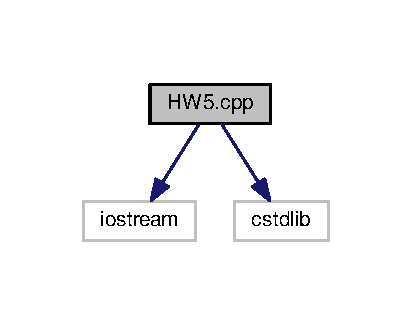
\includegraphics[width=198pt]{HW5_8cpp__incl}
\end{center}
\end{figure}
\subsection*{Functions}
\begin{DoxyCompactItemize}
\item 
void \hyperlink{HW5_8cpp_aafb8097a237228aa29c0dd0eadff9bec}{get\+\_\+numbers} (char a\mbox{[}$\,$\mbox{]}, int \&size)
\item 
void \hyperlink{HW5_8cpp_a46be15209729e924ce85ad73517ebd5e}{convert} (char a\mbox{[}$\,$\mbox{]}, int p\mbox{[}$\,$\mbox{]}, int size)
\item 
void \hyperlink{HW5_8cpp_a17a051d3d815b0bcfa726e40fad66b8d}{add} (int a\mbox{[}$\,$\mbox{]}, int b\mbox{[}$\,$\mbox{]}, int c\mbox{[}$\,$\mbox{]}, int size\+\_\+a, int size\+\_\+b)
\item 
void \hyperlink{HW5_8cpp_ada6e1f7ebdc3e2a275f5cee677ae339c}{output} (int c\mbox{[}$\,$\mbox{]}, int size)
\item 
int \hyperlink{HW5_8cpp_ae66f6b31b5ad750f1fe042a706a4e3d4}{main} ()
\end{DoxyCompactItemize}
\subsection*{Variables}
\begin{DoxyCompactItemize}
\item 
const int \hyperlink{HW5_8cpp_ab73857997d2049218b288a815758cb46}{L\+I\+M\+IT} = 100
\end{DoxyCompactItemize}


\subsection{Function Documentation}
\index{H\+W5.\+cpp@{H\+W5.\+cpp}!add@{add}}
\index{add@{add}!H\+W5.\+cpp@{H\+W5.\+cpp}}
\subsubsection[{\texorpdfstring{add(int a[], int b[], int c[], int size\+\_\+a, int size\+\_\+b)}{add(int a[], int b[], int c[], int size_a, int size_b)}}]{\setlength{\rightskip}{0pt plus 5cm}void add (
\begin{DoxyParamCaption}
\item[{int}]{a\mbox{[}$\,$\mbox{]}, }
\item[{int}]{b\mbox{[}$\,$\mbox{]}, }
\item[{int}]{c\mbox{[}$\,$\mbox{]}, }
\item[{int}]{size\+\_\+a, }
\item[{int}]{size\+\_\+b}
\end{DoxyParamCaption}
)}\hypertarget{HW5_8cpp_a17a051d3d815b0bcfa726e40fad66b8d}{}\label{HW5_8cpp_a17a051d3d815b0bcfa726e40fad66b8d}

\begin{DoxyCode}
96 \{
97    \textcolor{keywordtype}{int} num, carry\_over = 0;
98    \textcolor{keywordflow}{if}(size\_a > size\_b)
99    \{
100       \textcolor{keywordflow}{for}(\textcolor{keywordtype}{int} k = 0; k < size\_a-1; k++)
101       \{
102          \textcolor{keywordflow}{if}(k < size\_b)
103             num = a[k] + b[k] + carry\_over;
104          \textcolor{keywordflow}{else}
105             num = a[k] + carry\_over;
106          carry\_over = num/10; \textcolor{comment}{// carry\_over holds the number in the tens place                             
                                                                                                       }
107          num = num % 10; \textcolor{comment}{// num holds the number in the ones place                                         
                                                                                                       }
108          c[k] = num;
109       \}
110       c[size\_a-1] = a[size\_a-1] + carry\_over; \textcolor{comment}{// the last variable in the array holds the entire number
       (ones and tens place). Allows for the sum to be more than the LIMIT.                                }
111    \}
112    \textcolor{keywordflow}{else}
113    \{
114       \textcolor{keywordflow}{for}(\textcolor{keywordtype}{int} k = 0; k < size\_b-1; k++)
115       \{
116          \textcolor{keywordflow}{if}(k < size\_a)
117             num = a[k] + b[k] + carry\_over;
118          \textcolor{keywordflow}{else}
119             num = b[k] + carry\_over;
120         carry\_over = num/10;
121          num = num % 10;
122          c[k] = num;
123       \}
124       \textcolor{keywordflow}{if} (size\_a == size\_b) \textcolor{comment}{// if a and b are the same size, the a variable is added into the equation     
                                                                                                       }
125          c[size\_b-1] = b[size\_b-1] + a[size\_b-1] + carry\_over;
126       \textcolor{keywordflow}{else} \textcolor{comment}{// if b is bigger, the a variable is not added in                                               
                                                                                                       }
127          c[size\_b-1] = b[size\_b-1] + carry\_over;
128    \}
129 \}
\end{DoxyCode}
\index{H\+W5.\+cpp@{H\+W5.\+cpp}!convert@{convert}}
\index{convert@{convert}!H\+W5.\+cpp@{H\+W5.\+cpp}}
\subsubsection[{\texorpdfstring{convert(char a[], int p[], int size)}{convert(char a[], int p[], int size)}}]{\setlength{\rightskip}{0pt plus 5cm}void convert (
\begin{DoxyParamCaption}
\item[{char}]{a\mbox{[}$\,$\mbox{]}, }
\item[{int}]{p\mbox{[}$\,$\mbox{]}, }
\item[{int}]{size}
\end{DoxyParamCaption}
)}\hypertarget{HW5_8cpp_a46be15209729e924ce85ad73517ebd5e}{}\label{HW5_8cpp_a46be15209729e924ce85ad73517ebd5e}

\begin{DoxyCode}
84 \{
85    \textcolor{keywordtype}{char} character;
86    \textcolor{keywordtype}{int} x = 0;
87    \textcolor{keywordflow}{for}(\textcolor{keywordtype}{int} k = size-1; k >= 0; k--)
88    \{
89       character = a[k];
90       p[x] = int(character) - int(\textcolor{charliteral}{'0'});
91       x++;
92    \}
93 \}
\end{DoxyCode}
\index{H\+W5.\+cpp@{H\+W5.\+cpp}!get\+\_\+numbers@{get\+\_\+numbers}}
\index{get\+\_\+numbers@{get\+\_\+numbers}!H\+W5.\+cpp@{H\+W5.\+cpp}}
\subsubsection[{\texorpdfstring{get\+\_\+numbers(char a[], int \&size)}{get_numbers(char a[], int &size)}}]{\setlength{\rightskip}{0pt plus 5cm}void get\+\_\+numbers (
\begin{DoxyParamCaption}
\item[{char}]{a\mbox{[}$\,$\mbox{]}, }
\item[{int \&}]{size}
\end{DoxyParamCaption}
)}\hypertarget{HW5_8cpp_aafb8097a237228aa29c0dd0eadff9bec}{}\label{HW5_8cpp_aafb8097a237228aa29c0dd0eadff9bec}

\begin{DoxyCode}
62 \{
63    \textcolor{keywordtype}{char} character;
64    \textcolor{keywordtype}{int} x = 0;
65    cout << \textcolor{stringliteral}{"Enter a number (cannot be more than "} << \hyperlink{HW5_8cpp_ab73857997d2049218b288a815758cb46}{LIMIT} << \textcolor{stringliteral}{" digits). Type a period (.) after the
       number when you are finished entering: "};
66    cin >> character;
67    \textcolor{keywordflow}{while}(x <= LIMIT)
68    \{
69       \textcolor{keywordflow}{if}(character == \textcolor{charliteral}{'.'}) \textcolor{comment}{// stops function if a period is entered                                        
                                                                                                       }
70          \textcolor{keywordflow}{break};
71       \textcolor{keywordflow}{if}(x == LIMIT)
72       \{
73          cout << \textcolor{stringliteral}{"The integer entered exceeds the limit.The program has experienced integer overflow and
       will quit now.\(\backslash\)n"};
74          exit(1);
75       \}
76       a[x] = character; \textcolor{comment}{// assigns the entered value into an array variable                                
                                                                                                       }
77       cin >> character;
78       size++; \textcolor{comment}{// the size increases as numbers are added                                                   
                                                                                                       }
79       x++;
80    \}
81 \}
\end{DoxyCode}
\index{H\+W5.\+cpp@{H\+W5.\+cpp}!main@{main}}
\index{main@{main}!H\+W5.\+cpp@{H\+W5.\+cpp}}
\subsubsection[{\texorpdfstring{main()}{main()}}]{\setlength{\rightskip}{0pt plus 5cm}int main (
\begin{DoxyParamCaption}
{}
\end{DoxyParamCaption}
)}\hypertarget{HW5_8cpp_ae66f6b31b5ad750f1fe042a706a4e3d4}{}\label{HW5_8cpp_ae66f6b31b5ad750f1fe042a706a4e3d4}

\begin{DoxyCode}
25 \{
26    \textcolor{keywordtype}{char} arrayA[\hyperlink{HW5_8cpp_ab73857997d2049218b288a815758cb46}{LIMIT}], arrayB[\hyperlink{HW5_8cpp_ab73857997d2049218b288a815758cb46}{LIMIT}], choice;
27    \textcolor{keywordflow}{do}
28    \{
29       \textcolor{keywordtype}{int} *a, *b, *c, size\_a = 0, size\_b = 0, size\_c = 0;
30 
31       \hyperlink{HW5_8cpp_aafb8097a237228aa29c0dd0eadff9bec}{get\_numbers}(arrayA, size\_a); \textcolor{comment}{// fills arrayA with a list of numbers                       
                                                                                                                  }
32       \hyperlink{HW5_8cpp_aafb8097a237228aa29c0dd0eadff9bec}{get\_numbers}(arrayB, size\_b);
33 
34       a = \textcolor{keyword}{new} \textcolor{keywordtype}{int}[size\_a]; \textcolor{comment}{// makes a dynamic array called a                                               
                                                                                                       }
35       b = \textcolor{keyword}{new} \textcolor{keywordtype}{int}[size\_b];
36       \textcolor{keywordflow}{if}(size\_a > size\_b)
37       \{
38          c = \textcolor{keyword}{new} \textcolor{keywordtype}{int}[size\_a];
39          size\_c = size\_a;
40       \}
41       \textcolor{keywordflow}{else}
42       \{
43          c = \textcolor{keyword}{new} \textcolor{keywordtype}{int}[size\_b];
44          size\_c = size\_b;
45       \}
46 
47       \hyperlink{HW5_8cpp_a46be15209729e924ce85ad73517ebd5e}{convert}(arrayA, a, size\_a); \textcolor{comment}{// copies arrayA's values to dynamic array a in reverse order     
                                                                                                              }
48       \hyperlink{HW5_8cpp_a46be15209729e924ce85ad73517ebd5e}{convert}(arrayB, b, size\_b);
49       \hyperlink{HW5_8cpp_a17a051d3d815b0bcfa726e40fad66b8d}{add}(a, b, c, size\_a, size\_b); \textcolor{comment}{// adds the two values from a and b, and puts the new value into c  
                                                                                                          }
50       \hyperlink{HW5_8cpp_ada6e1f7ebdc3e2a275f5cee677ae339c}{output}(c, size\_c); \textcolor{comment}{// displays values in c in reverse order (the sum of arrayA and arrayB)     
                                                                                                             }
51 
52       \textcolor{keyword}{delete} []a; \textcolor{comment}{// deletes the dynamic arrays                                                            
                                                                                                       }
53       \textcolor{keyword}{delete} []b;
54       \textcolor{keyword}{delete} []c;
55       cout << \textcolor{stringliteral}{"Would you like to do more addition? Enter y or Y to continue, and any other character to
       quit: "};
56       cin >> choice;
57    \} \textcolor{keywordflow}{while}(choice == \textcolor{charliteral}{'y'} || choice == \textcolor{charliteral}{'Y'});
58    \textcolor{keywordflow}{return} 0;
59 \}
\end{DoxyCode}


Here is the call graph for this function\+:
\nopagebreak
\begin{figure}[H]
\begin{center}
\leavevmode
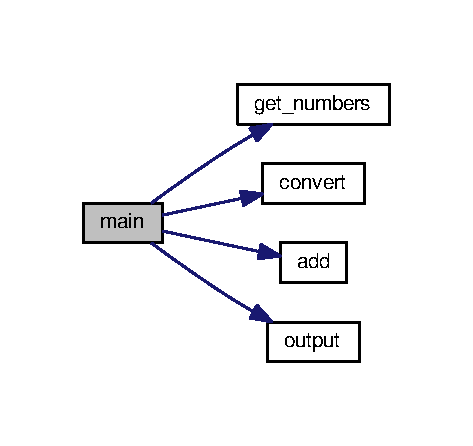
\includegraphics[width=227pt]{HW5_8cpp_ae66f6b31b5ad750f1fe042a706a4e3d4_cgraph}
\end{center}
\end{figure}


\index{H\+W5.\+cpp@{H\+W5.\+cpp}!output@{output}}
\index{output@{output}!H\+W5.\+cpp@{H\+W5.\+cpp}}
\subsubsection[{\texorpdfstring{output(int c[], int size)}{output(int c[], int size)}}]{\setlength{\rightskip}{0pt plus 5cm}void output (
\begin{DoxyParamCaption}
\item[{int}]{c\mbox{[}$\,$\mbox{]}, }
\item[{int}]{size}
\end{DoxyParamCaption}
)}\hypertarget{HW5_8cpp_ada6e1f7ebdc3e2a275f5cee677ae339c}{}\label{HW5_8cpp_ada6e1f7ebdc3e2a275f5cee677ae339c}

\begin{DoxyCode}
132 \{
133    cout << \textcolor{stringliteral}{"The sum of those two numbers is: "};
134    \textcolor{keywordflow}{for}(\textcolor{keywordtype}{int} k = size-1; k >= 0; k--) \textcolor{comment}{// outputs the values in c in reverse order                            
                                                                                                       }
135       cout << c[k];
136    cout << endl;
137 \}
\end{DoxyCode}


\subsection{Variable Documentation}
\index{H\+W5.\+cpp@{H\+W5.\+cpp}!L\+I\+M\+IT@{L\+I\+M\+IT}}
\index{L\+I\+M\+IT@{L\+I\+M\+IT}!H\+W5.\+cpp@{H\+W5.\+cpp}}
\subsubsection[{\texorpdfstring{L\+I\+M\+IT}{LIMIT}}]{\setlength{\rightskip}{0pt plus 5cm}const int L\+I\+M\+IT = 100}\hypertarget{HW5_8cpp_ab73857997d2049218b288a815758cb46}{}\label{HW5_8cpp_ab73857997d2049218b288a815758cb46}

%--- End generated contents ---

% Index
\backmatter
\newpage
\phantomsection
\clearemptydoublepage
\addcontentsline{toc}{chapter}{Index}
\printindex

\end{document}
